\documentclass{article}
\usepackage{tikz}
\usepackage{verbatim}
\usepackage{cprotect}
\usepackage{fullpage}

\begin{document}
%\begin{tikzpicture}
%\draw (0,2) rectangle (2, 4);
%\draw[blue] (1.8,2.2) rectangle (4, 2);
%\draw[red] (4,4) rectangle (6, 0);
%\end{tikzpicture}

%{\Large \textbf{$>$ scatter.smooth(mtcars[ , c(1, 2)])}};
\begin{figure}
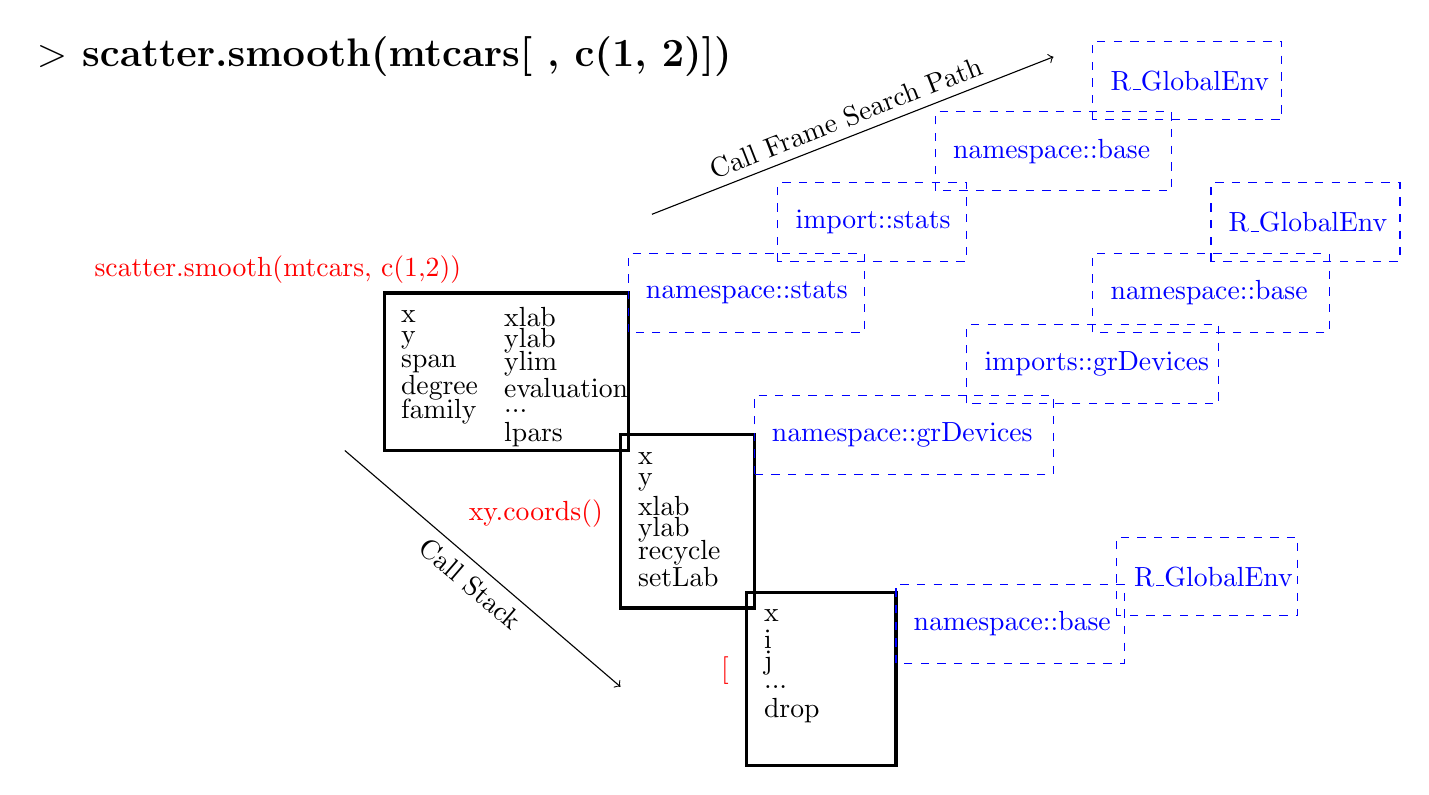
\begin{tikzpicture}
%\draw (0,9) node[anchor=east] {\Large \textbf{$>$ scatter.smooth(mtcars[ , c(1, 2)])}};
\draw (0,9) node {\Large \textbf{$>$ scatter.smooth(mtcars[ , c(1, 2)])}};

\begin{scope}[very thick]
\draw (0,6) rectangle (3.1, 4)   ;   %scatter.smooth
\draw (3.0,4.2) rectangle (4.7, 2); %xy.coords
\draw (4.6,2.2) rectangle (6.5, 0); %[
\end{scope}

\draw [->] (-.5,4) -- (3.0, 1)
     node [midway,sloped,below] {Call Stack};


%anchor=west
\begin{scope}[anchor=east,color=red]
\draw (1.1, 6.3) node {scatter.smooth(mtcars, c(1,2))} ;
%\draw (-.1, 5.1) node {scatter.smooth} ;
\draw (2.9, 3.2) node {xy.coords()} ;
\draw (4.5, 1.2) node {[} ;
\end{scope}
\begin{scope}[anchor=west]
\draw (.09, 5.7) node {x} ;
\draw (.09, 5.4) node {y} ;
\draw (.09, 5.1) node {span};
\draw (.09, 4.8) node {degree};
\draw (.09, 4.5) node {family};
\draw (1.4, 5.7) node {xlab};
\draw (1.4, 5.4) node {ylab};
\draw (1.4, 5.1) node {ylim};
\draw (1.4, 4.8) node {evaluation};
\draw (1.4, 4.5) node {...};
\draw (1.4, 4.2) node {lpars};
\end{scope}
\begin{scope}[anchor=west]
\draw (3.1, 3.9) node {x} ;
\draw (3.1, 3.6) node {y} ;
\draw (3.1, 3.3) node {xlab};
\draw (3.1, 3.0) node {ylab};
\draw (3.1, 2.7) node {recycle};
\draw (3.1, 2.4) node {setLab};
\end{scope}
\begin{scope}[anchor=west]
\draw (4.7, 1.9) node {x} ;
\draw (4.7, 1.6) node {i} ;
\draw (4.7, 1.3) node {j};
\draw (4.7, 1.0) node {...};
\draw (4.7, .7) node {drop};
\end{scope}

\draw [->] (3.4,7.) -- (8.5, 9.)  node [above,midway,sloped] {Call Frame Search Path};
\begin{scope}[dashed,color=blue]
\draw (3.1,5.5) rectangle (6.1, 6.5);
\draw (3.2,6) node[anchor=west] {namespace::stats};
\draw (5.,6.4) rectangle (7.4, 7.4);
\draw (5.1,6.9) node[anchor=west] {import::stats};

\draw (7.,7.3) rectangle (10.0, 8.3);
\draw (7.1,7.8) node[anchor=west] {namespace::base};
\draw (9.,8.2) rectangle (11.4, 9.2);
\draw (9.1,8.7) node[anchor=west] {R\_GlobalEnv};


\draw (4.7,3.7) rectangle (8.5, 4.7);
\draw (4.8,4.2) node[anchor=west] {namespace::grDevices};
\draw (7.4,4.6) rectangle (10.6, 5.6);
\draw (7.5,5.1) node[anchor=west] {imports::grDevices};
\draw (9.,5.5) rectangle (12., 6.5);
\draw (9.1,6.0) node[anchor=west] {namespace::base};
\draw (10.5,6.4) rectangle (12.9, 7.4);
\draw (10.6,6.9) node[anchor=west] {R\_GlobalEnv};

%\draw[blue] (3.0,4.2) rectangle (4.8, 2);
%\draw[red] (4.6,2.2) rectangle (6.6, 0);

% [
\draw (6.5,1.3) rectangle (9.4, 2.3);
\draw (6.6,1.8) node[anchor=west] {namespace::base};
\draw (9.3,1.9) rectangle (11.6, 2.9);
\draw (9.4,2.4) node[anchor=west] {R\_GlobalEnv};
\end{scope}
\end{tikzpicture}
\cprotect\caption[The Call Stack, Call Frames and their Search Paths]{\textbf{The Call Stack, Call Frames and their Search Paths.}
This shows the call stack for \verb!scatter.smooth(mtcars[, c(1, 2)])!.
scatter.smooth() calls xy.coords() and finally the argument for x in 
scatter.smooth is needed. Due to R's lazy evaluation, this is evaluated next,
hence the call the \verb![(mtcars, c(1, 2))!.
Within each of the three call frames, 
R searches for symbols by looking first in the 
call frame and then in its parent environment, and its parent environment,
and so on.
These  environments are displayed moving from left to right and show
the search through packages and their imports and their parents.
Afer \verb|R_GlobalEnv|, the search continues along the regular search path,
i.e., the packages loaded on the seach path via require() and library().
}
\end{figure}
\end{document}
